\begin{figure}[tb]
	\includegraphics[width=\textwidth]{images/pml/oqe_schemat.png}
	\caption{Schematyczne przedstawienie analizowanej struktury warstwowej i przybliżanego przy pomocy modelu ośrodka efektywnego ośrodka PML}
	\label{fig:pml-multilay-schem}
\end{figure}

Porównując ogólną postać PML podaną w równaniu (\ref{eq:general-pml-form}) z modelem ośrodka efektywnego przedstawionym w podrozdziale \ref{subart:effmedium} można zaproponować przybliżenie ośrodka typu PML przy pomocy struktury warstwowej o odpowiednich właściwościach efektywnych. W szczególności dla uproszczenia analizy skupimy się na polaryzacji TM, dla której istotnymi składowymi tensorów opisujących własności materiałowe są:$\varepsilon_x$,$\mu_y$i $\varepsilon_z$. Ze względu na ograniczenia używanego modelu ośrodka efektywnego, zgodnie ze schmatem na rysunku \ref{fig:pml-multilay-schem} $\varepsilon_x=\varepsilon_y$, oraz $\mu_x=\mu_y$. Ponownie odwołując się do granicy między ośrodkami przedstawione na rysunku \ref{fig:pml-multilay-schem} warunki dla których wielowarstwa będzie efektywnie spełniać rolę PML przedstawiają się następująco:
\begin{equation}
	f\cdot \varepsilon_{w1} + (1-f)\cdot \varepsilon_{w2} = s \cdot \varepsilon_1,
	\label{eq:oqe4}
\end{equation}

\begin{equation}
	[f\cdot \varepsilon_{w1}^{-1}+(1-f)\varepsilon_{w2}^{-1}]^-1=s^{-1}\cdot \varepsilon_1,
	\label{eq:oqe5}
\end{equation}

\begin{equation}
	f\cdot \mu_{w1} + (1-f)\cdot \mu_{w2} = s \cdot \mu_1,
	\label{eq:oqe6}
\end{equation}
gdzie przez $f$ oznaczony został współczynnik wypełnienia, równy ułamkowi przestrzeni wielowarstwy zajmowanemu przez materiał $w1$. Odpowiednie warunki dla polaryzacji TE to:
\begin{equation}
	\varepsilon_{w1}=\rho \frac{\varepsilon_1 \cdot s}{f\cdot \rho + (1 -f) },
	\label{eq:te-eps1}
\end{equation}

\begin{equation}
	\varepsilon_{w2}=\frac{\varepsilon_1 \cdot s}{f\cdot \rho + (1-f)},
	\label{eq:te-eps2}
\end{equation}
gdzie
\begin{equation}
	\rho = 1+\frac{s^2-1 \pm \sqrt{(s^2-1)(s^2-(2f-1)^1)}}{2f(1-f)}.
	\label{eq:te-rho}
\end{equation}

\begin{figure}[tb]
	\includegraphics[width=\textwidth]{images/pml/oqe_materials.png}
	\caption{Zależność przenikalności elektrycznej materiałów tworzących UPML (w lewej kolumnie $\varepsilon_{w1}$, w prawej $\varepsilon_{w2}$) w funkcji współczynnika wypełnienia i urojonej części parametru $s$ (założono $\textrm{Re(s)=1}$. Górny wiersz na wykresach (a) i (b) prezentuje zależności części rzeczywistych, dolny na wykresach (c) i (d) części urojonych przenikalności elektrycznych. Ujemne wartości $\varepsilon$ na wykresach (c) i (d) odpowiadają materiałom ze wzmocnieniem optycznym. }
	\label{fig:upml-eps-s-f}
\end{figure}

Wykresy na rysunku \ref{fig:upml-eps-s-f} prezentują wyniki obliczonych (\ref{eq:te-eps1}) i (\ref{eq:te-eps2}) jako funkcję współczynnika wypełnienia $f$ i parametru $s$, dla którego przyjęto $s=1+\alpha i$. Używamy rozwiązań dla (\ref{eq:te-rho}) z $|\rho|>1$. Podobne wyrażenia jak (\ref{eq:oqe4}) i (\ref{oqe5}) można wypisać i rozwiązać dla $\mu_{w1}$ i $\mu_{s2}$. W przypadku gdy $\varepsilon_1=\mu_1$ otrzymujemy $\varepsilon_{w1}=\mu_{w1}$ i $\varepsilon_{w2}=\mu_{w2}$. 

Zależność współczynnika odbicia od kąta padania, oraz grubości komórki elementarnej wielowarstwy przedstawia wykres na rysunku \ref{fig:oqe3}. Ze względu na umieszczenie idealnego przewodnika za wielowarstwą współczynnik odbicia łączy w sobie część odbijaną od wielowarstwy, jak i transmitowaną przez wielowarstwę i odbijaną od zwierciadła z PEC. Analizując wykres \ref{fig:oqe3} możemy zauważyć, że wraz ze wzrostem $\frac{a}{\lambda}$ zmniejsza się współczynnik odbicia fal propagujących się $\frac{k_x}{k_0}<1$. Wynika to z faktu jednoczesnego zwiększania grubości warstwy pochłaniającej, więc jest przedewszystkim związane ze zmniejszeniem transmisji przez wielowarstwę. W przypadku fal ewanescętnych $\frac{k_x}{k_0}>1$ obserwujemy wzrost współczynnika odbicia. Można to interpretować jako odbicie od pierwszej warstwy wynikające z niespełnienia warunków homogenizacji (przybliżenie ośrodka efektywnego zakłada $\frac{a}{\lambda} \to 0$) przez strukturę. Dlatego wzrost jest większy dla większej części urojonej współczynnika $s$, skutkującej większą różnicą współczynników załamania na granicy pierwszej warstwy i powietrza.

\begin{figure}[tb]
	\includegraphics[width=\textwidth]{images/pml/fig3.png}
	\caption{Zależność natężeniowego współczynnika odbicia od kąta padania i okresu wielowarstwy dla struktury zgodniej ze schmatem na rysunuku \ref{fig:pml-multilay-schem}, dla $N=5$ par warstw, przy współczynniku wypełnienia $f=0.6$. Wysunek po lewej (a) przedstawia wyniki dla $s=1+0.5i$, wykres po prawej przedstawia wyniki dla $s=1+5i$.}
	\label{fig:oqe3}
\end{figure}

Przedstawione wyniki możliwe są do osiągnięcia przy pomocy materiałów wykazujących szczególne własności elektryczne i magnetyczne, w szczególności obliczenia zakładały zespoloną przenikalność magnetyczną, oraz zysk optyczny. Dla $s=1+5i$ możliwe jest uzyskanie warstwy PML o całkowitej grubości $5\cdot a \approx \frac{\lambda}{20}$ wykazującej natężeniowy współczynnik odbicia ok -30dB dla szerokiego zakresu kątów padających fal płaskich.

W przypadku oświetlenia wielowarstwy przy pomocy polaryzacji TM jeden ze współczynników przenikalności magnetycznej może zostać ustalony w sposób arbitralny. W szczególności możemy więc założyć $\mu_{w2}=1$, ponieważ większość materiałów spotykanych w przyrodzie charakteryzuje się taką wartością dla częstotliwości optycznych. Drugą przenikalność magentyczną możemy wyznaczyć przy pomocy wzoru \ref{eq:oqe6}. Część rzeczywista $\textrm{Re}(\mu_{w1})=1$, a zależność części urojonej $\textrm{Im}(\mu_{w1})$ od części urojonej współczynnika $s$, oraz współczynnika wypełnienia przedstawia wykres \ref{fig:im-mu1}. Na podstawie przywołanego wykresu możemy zauważyć, że wysoki współczynnik wypełnienia, oraz wykorzystanie małej części urojonej $s$ skutkują małymi wartościami $\textrm{Im}(\mu_{w1})$, jest to dla nas istotne ponieważ korzystając z realnych materiałów będziemy zmuszeni przybliżyć te wartość przez $0$.

W przypadku zastosowania nie numerycznego należy zaniedbać własności magnetyczne materiałów $\mu=1$, oraz zysk optyczny $\textrm{Im}(\varepsilon)\ge0$. Wyniki dla obu polarizacji po zasotosowaniu się do wymienionych przybliżeń przedstawiają wykresy na rysunku \ref{fig:pml-real-ref}. Zaproponowany absorber skład się z materiału stratnego, oraz warstw charakteryzujących się przenikalnością elektryczną mniejszą od 1. Przedstawione wyniki obliczeń wskazują, że w wyniku poczynionych założeń efektywność pracy wielowarstwy jako struktury PML znacznie różni się w zależności od polaryzacji. Niższe wartości współczynnika odbicia uzyskujemy w tym przypadku dla polaryzacji TE. Wysokie współczynniki odbicia pojawiają się jednak jedynia dla kątów padania bliskich $90^{\circ}$, co jest charakterystyczne dla UPML.


\begin{SCfigure}
	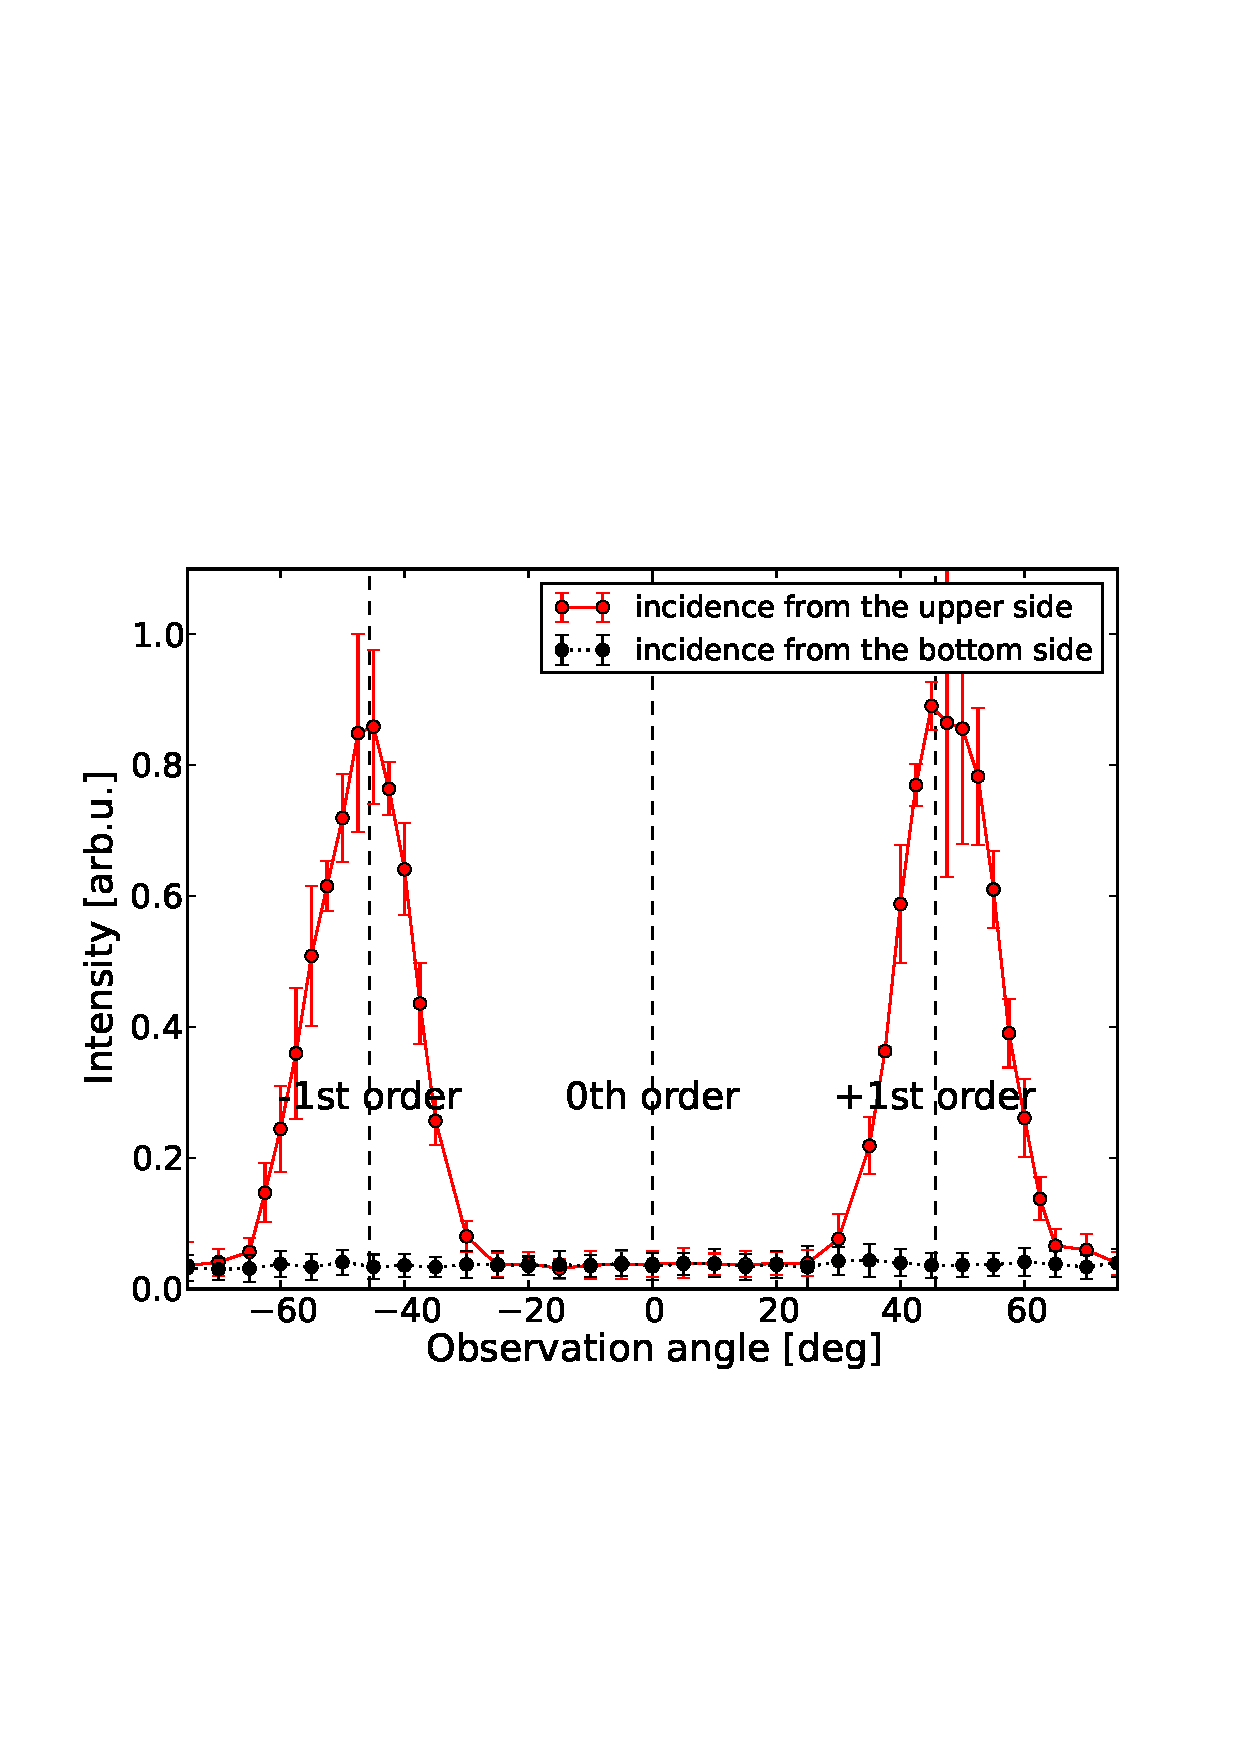
\includegraphics[width=0.6\textwidth]{images/pml/fig4.png}
	\caption{Zależność części urojonej przenikalności magnetycznej jednego z materiałów $\mu_{w1}$, od części urojonej współczynnika $s$ i współczynnika wypełnienia $f$ w przypadku gdy założono $\mu_{w2}=1$}
	\label{fig:im-mu1}
\end{SCfigure}



\begin{figure}[tb]
	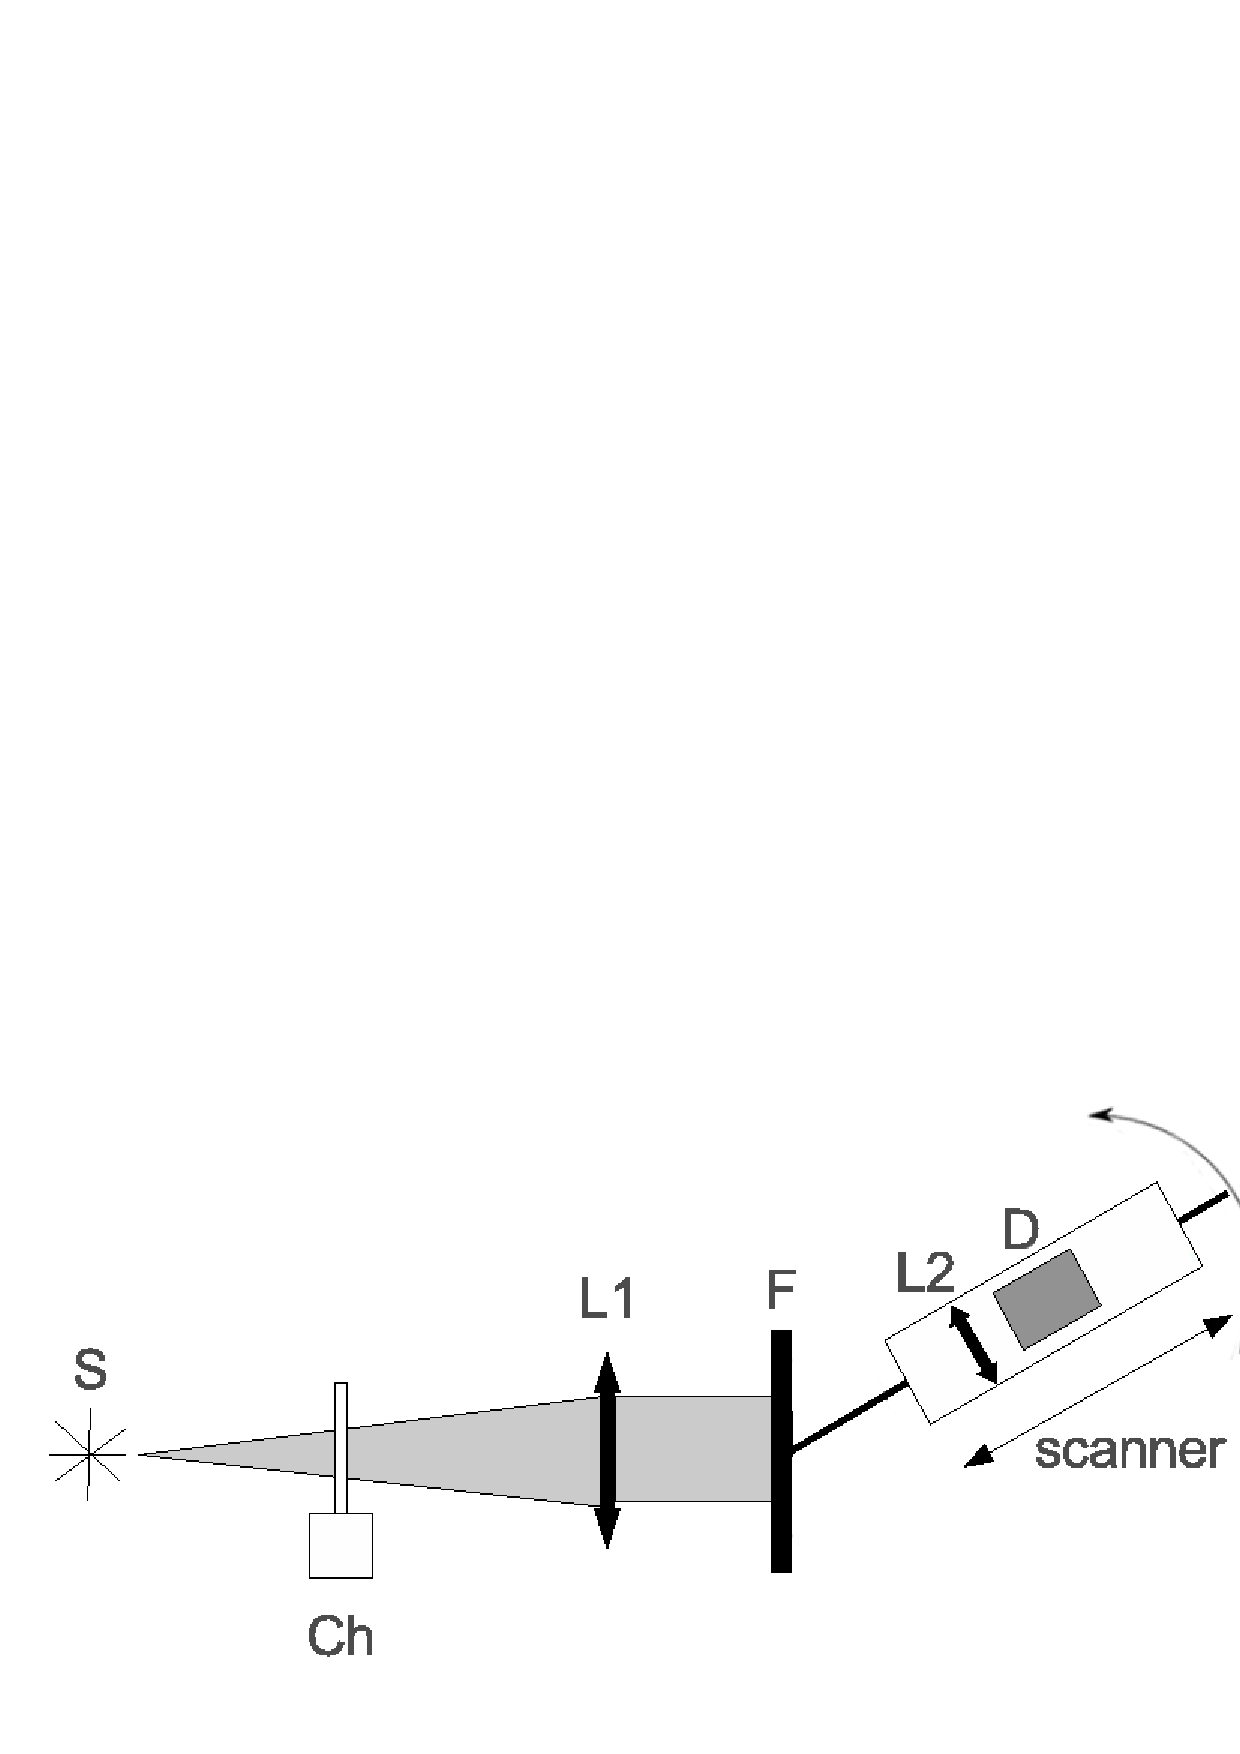
\includegraphics[width=\textwidth]{images/pml/fig5.png}
	\caption{Zależność natężeniowego współczynnika odbicia $R$, od kąta padania i grubości warstw dla wielowarstwy składającej się z $N=5$ okresów, dla $s=1+5i$ i $f=0.6$. Spełniając założenie, że $\mu_{w2}=1$ (a,c), oraz $\mu_{w1}=\mu_{w2}=1$, $\textrm{Im}(\varepsilon_1)\ge 0 $ i $\textrm{Im}(\varepsilon_2)\ge 0 $ (b,d). Wyniki dla polaryzacji TM (a,b) oraz TE (c,d). Przenikalnośc elektryczna $\varepsilon_{w1}=1.474+1.017i$.}
	\label{fig:pml-real-ref}
\end{figure}

\begin{figure}[tb]
	\centering
	\includegraphics[width=0.8\textwidth]{images/pml/oqe_trans_refl.png}
	\caption{Współczynnik transmisji (linia ciągła) i odbicia (linia przerywana) dla wielowarstwy złożonej z $SiO_2$/$NaCl$ zaprojekowanej dla oświetlenia długością fali 8~$\mu$m, dla której współczynniki załamania $n_{\textrm{SiO}_2}=0.41+0.32i$, $n_{\textrm{NaCl}}=1.51$. Współczynnik wypełnienia struktury przez $SiO_2$ wynosi $f=0.56$, $a=200nm$. Rozważone zostały stosy o $N=10,100,400$.}
	\label{fig:oqe-trans-refl}
\end{figure}

\begin{figure}[tb]
	\includegraphics[width=\textwidth]{images/pml/oqe_coreshell.png}
\end{figure}


